\iffalse
\let\negmedspace\undefined
\let\negthickspace\undefined
\documentclass[journal,12pt,twocolumn]{IEEEtran}
\usepackage{cite}
\usepackage{amsmath,amssymb,amsfonts,amsthm}
\usepackage{algorithmic}
\usepackage{graphicx}
\usepackage{textcomp}
\usepackage{xcolor}
\usepackage{txfonts}
\usepackage{listings}
\usepackage{enumitem}
\usepackage{mathtools}
\usepackage{gensymb}
\usepackage{comment}
\usepackage[breaklinks=true]{hyperref}
\usepackage{tkz-euclide} 
\usepackage{listings}
\usepackage{gvv}                                        
\def\inputGnumericTable{}                                 
\usepackage[latin1]{inputenc}                                
\usepackage{color}                                            
\usepackage{array}                                            
\usepackage{longtable}                                       
\usepackage{calc}                                             
\usepackage{multirow}                                         
\usepackage{hhline}                                           
\usepackage{ifthen}                                           
\usepackage{lscape}
\newtheorem{theorem}{Theorem}[section]
\newtheorem{problem}{Problem}
\newtheorem{proposition}{Proposition}[section]
\newtheorem{lemma}{Lemma}[section]
\newtheorem{corollary}[theorem]{Corollary}
\newtheorem{example}{Example}[section]
\newtheorem{definition}[problem]{Definition}
\newcommand{\BEQA}{\begin{eqnarray}}
\newcommand{\EEQA}{\end{eqnarray}}
\newcommand{\define}{\stackrel{\triangle}{=}}
\theoremstyle{remark}
\newtheorem{rem}{Remark}
\begin{document}
\parindent 0px
\bibliographystyle{IEEEtran}
\title{ASSIGNMENT11.15\_13Q}
\author{EE22BTECH11219 - Sai Sujan Rada$^{}$% <-this % stops a space
}
\maketitle
\newpage
\bigskip
\section*{QUESTION}
Given below are some functions of x and t to 
represent the displacement (transverse
or longitudinal) of an elastic wave. State which of these represents \brak i travelling
wave, \brak {ii} a stationary wave or \brak {iii} none at all: \\
\begin{enumerate}
\item $y = 2\cos \brak{3x} \sin \brak{10t}$
\item $y=2\sqrt{x-vt}$
\item $y = 3\sin \brak{5x - 0.5t} + 4\cos \brak{5x - 0.5t}$
\item $y = \cos x \sin t + \cos 2x \sin 2t$
\end{enumerate}
\solution 
\fi
\begin{table}[htbp]
    \centering
    \def\arraystretch{1.5}
    \begin{tabular}{|p{4cm}|p{4cm}|}
    \hline
TRAVELLING WAVE  & STATIONARY WAVE \\ \hline
    $y \brak{x,t} =A \sin  \brak{kx \pm \omega t} $ & $y\brak{ x,t }=A\sin kx\cos \omega t $ \\   \hline
    \hline
PARAMETERS  & DEFINITION  \\  \hline
$A$    &  Amplitude  \\ \hline
 $\omega$  & Angular Velocity  \\  \hline
 $x$    & Position  \\  \hline
 $k$    & Wavenumber    \\  \hline 
    \end{tabular}
    \caption{Travelling wave $vs$ Stationary wave}
    \label{tab:table1}
\end{table}

Let us assume an equation:
\begin{align}
y=A(x)\cos \brak{\omega t+\phi\brak {x}}
\end{align}
\begin{table}[htbp]
    \centering
    \def\arraystretch{1.5}
    \begin{tabular}{|p{4cm}|p{4cm}|}
    \hline
STATIONARY WAVE CONDITION & TRAVELLING WAVE CONDITION \\ \hline
        \brak 1 $A(x)$ should be a function of position x, and it can be expressed as $A(x)=A_{0}cos(\omega t+\alpha)$ where $A_{0}$ is a constant, $k$ is the wavenumber, $x$ is the position and $\alpha$ is a phase constant. & 
        \brak 1 $A(x)$ should be a constant, and it can be expressed as $A(x)=A_{0}$ where $A_{0}$ is a constant number. \\ \hline

        \brak 2 $\phi (x)$ can be expressed as $\phi (x)=c$ where c is a constant. &
        \brak 2 $\phi (x)$ represents a linear expression in x, and it can be expressed as $\phi (x)=kx+\theta$ where k is the wavenumber and $\theta$ is the phaseconstant. \\ \hline
\end{tabular}
    \caption{Travelling wave $vs$ Stationary wave}
    \label{tab:table1}
\end{table}

\begin{figure}[ht]
                        \centering
                        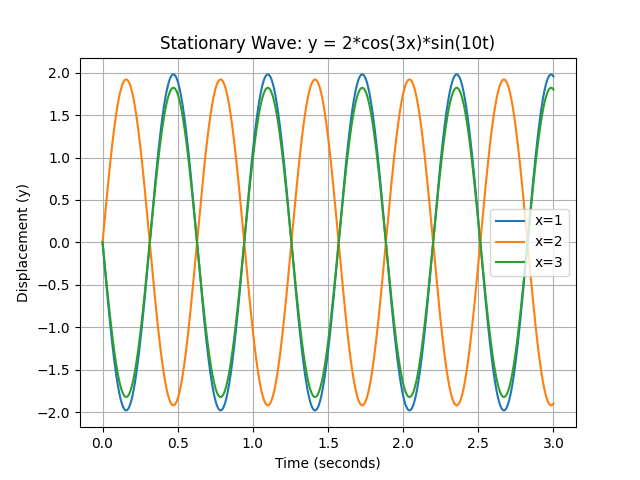
\includegraphics[width=\columnwidth]{figs/a.png}
                        \caption{DIPLACEMENT $vs$ TIME-graph1}
                        \label{fig:1}
\end{figure}
\begin{figure}[ht]
                            \centering
                            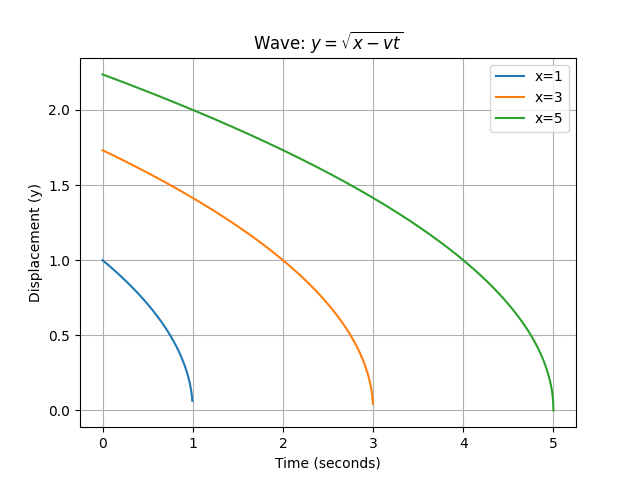
\includegraphics[width=\columnwidth]{figs/b.png}
                            \caption{DIPLACEMENT $vs$ TIME-graph2}
                            \label{fig:2}
\end{figure}   
\begin{figure}[ht]
                             \centering
                             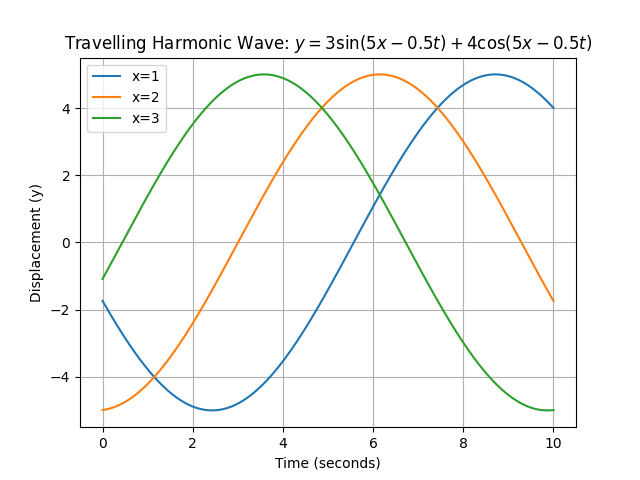
\includegraphics[width=\columnwidth]{figs/c.png}
                             \caption{DIPLACEMENT $vs$ TIME-graph3}
                             \label{fig:3}
\end{figure}
\begin{figure}[ht]
                            \centering
                            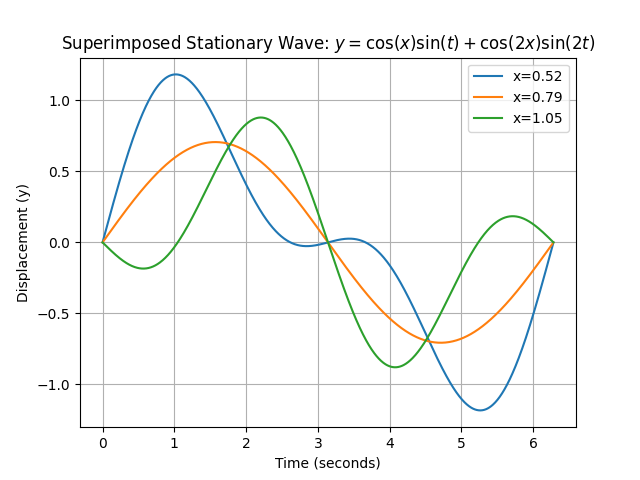
\includegraphics[width=\columnwidth]{figs/d.png}
                            \caption{DIPLACEMENT $vs$ TIME-graph4}
                            \label{fig:4}
\end{figure}
\figref{fig:1} and \figref{fig:3} are self explanatory for stationary and travelling waves.
\figref{fig:2} and \figref{fig:4} are neither stationary nor travelling waves. 
